\documentclass[10pt,twocolumn]{article}

\usepackage[margin=0.75in]{geometry}
\usepackage{fontspec}
\setmainfont{TeX Gyre Termes}
\setsansfont{TeX Gyre Heros}
\setmonofont{Latin Modern Mono}
\usepackage{microtype}
\usepackage{graphicx}
\usepackage{xcolor}
\usepackage[table]{xcolor}
\usepackage{booktabs}
\usepackage{threeparttable}
\usepackage{tabularx}
\usepackage{array}
\usepackage{caption}
\usepackage{tikz}
\usetikzlibrary{arrows.meta,positioning,fit,backgrounds,shapes.geometric,calc}
\usepackage{xr-hyper}
\usepackage[hidelinks]{hyperref}
\externaldocument[supp:]{supplemental_material}

\setlength{\columnsep}{0.24in}
\setlength{\parskip}{0pt}
\setlength{\parindent}{1em}
\captionsetup{font=small,labelfont=bf}

\newcommand{\best}[1]{\textbf{#1}}

\begin{document}

\title{\textbf{A Controlled Study of HyDE-Style Query Expansion}\\
\textbf{for Multi-Hop Evidence Acquisition}}

\author{Anonymous submission}

\date{}

\maketitle

\begin{abstract}
Retrieval-augmented generation (RAG) often fails on multi-hop question answering when retrieval omits part of the required supporting evidence. We present a controlled diagnostic study of HyDE-style document-like query expansion for this retrieval bottleneck, rather than a new retriever architecture. In the studied fixed-depth, training-free protocol, an LLM generates a concise hypothetical supporting passage for each question; the question and passage are concatenated for dense retrieval, and the reader receives only the question and retrieved corpus evidence and is instructed to answer from that evidence. On the 500-example HotpotQA processed split, HyDE-style RAG improves all-support hit@10 from 0.6300 to 0.8680 and answer F1 from 0.7199 to 0.8105 over one-step Dense RAG. A matched-call query-reformulation control reaches 0.6180 all-support hit@10 and 0.7130 F1, indicating that one additional query-side LLM call alone does not explain the gain. A secondary 2WikiMultihopQA evaluation shows the same direction relative to dense, BM25, and hybrid retrieval. The effect remains positive with a no-retuning BGE-base encoder check and under retrieval stress tests of up to 100k passages. Under equal generation budgets, document-like passages consistently outperform direct rewriting and question decomposition, while their comparison with keyword/entity expansion is dataset-dependent. Overall, the paper's mechanism conclusion is limited to retrieval-stage supporting-title and paragraph-text acquisition under the evaluated processed local-corpus protocol.
\end{abstract}

\section{Introduction}
\label{sec:introduction}

Retrieval-augmented generation (RAG) grounds language-model answers in external evidence, but multi-hop question answering stresses this design. A question may require linking entities, comparing facts, or combining evidence from multiple documents. If retrieval returns only part of the supporting evidence, the reader may still fail even when the answer is straightforward from the full evidence set. Supporting-title completeness, checked against supporting paragraph text when the processed artifacts expose it, is therefore a natural diagnostic for multi-hop RAG.

Prior work addresses multi-hop evidence acquisition with more adaptive retrieval and reasoning. IRCoT-style methods interleave reasoning traces with retrieval, and agentic or self-reflective RAG systems can decide when to retrieve, critique, or revise outputs. We ask a narrower empirical question: under a fixed-depth, training-free protocol, when does HyDE-style generative expansion improve complete supporting-title and paragraph-text retrieval without an open-ended retrieval loop?

Building on HyDE rather than proposing a new retriever architecture, we examine document-like generative query expansion in this fixed-depth protocol. The evaluated pipeline generates a concise hypothetical supporting passage, retrieves with the question plus that passage as the dense query, and then applies an evidence-grounded short-answer reader. Unlike direct query rewriting, the generated text is document-like and may expose likely entities, relations, and answer types for dense retrieval.

The main empirical pattern is evidence-driven. On HotpotQA \texttt{test\_subsampled}, HyDE-style RAG raises all-support hit@10 to 0.8680 and mean supporting-title recall@10 to 0.9280, with reader EM/F1 of 0.6840/0.8105. These values exceed the implemented lightweight retrieval baselines and diagnostic controls in our fixed local-corpus protocol, including dense, BM25, hybrid, rule-based multi-query, rule-based iterative retrieval, and matched-call query reformulation. We do not treat these author-implemented controls as faithful reproductions of all neighboring published systems. A secondary guarded canonicalization diagnostic produces only a small, statistically non-significant answer-format change, so we treat it as exploratory post-processing rather than as a primary accuracy contribution.

This controlled study makes three empirical contributions. First, it shows that HyDE-style document-like expansion can improve complete supporting-title retrieval in a fixed-depth multi-hop RAG protocol, with matching paragraph-text audit results and answer gains reported for the fixed reader used in the main evaluation. Second, it isolates competing explanations through matched-call, query-composition, paired, supporting-title and paragraph-text, answer-string-overlap, strict equal-budget query-form, and top-$k$ sensitivity diagnostics; these controls reduce explanations based only on an extra LLM call, retained question text, ordinary direct rewriting, generated length, title-level scoring artifacts, or a single cutoff at rank 10. Third, it characterizes boundary conditions through answer-overlap, gold-content scrubbing, stronger-encoder, corpus-scale leakage and hard-negative audits, and targeted reader checks, showing that answer-like generated content, high-information keyword expansion, encoder strength, corpus scale and difficulty, sentence-level annotation limits, and reader choice affect how far the mechanism claim should generalize. The resulting claim is intentionally retrieval-stage and diagnostic: document-like expansion improves complete supporting-title and paragraph-text acquisition over direct reformulation and question decomposition under the evaluated protocol, while its advantage over keyword/entity expansion is dataset-dependent. We additionally report guarded canonicalization only as a secondary answer-format risk analysis.

\section{Related Work}
\label{sec:related_work}

\subsection{Retrieval-Augmented Generation and Dense Retrieval}
\label{sec:rw_rag_dense}

Retrieval-augmented generation (RAG) grounds language-model outputs in external evidence rather than relying only on parametric memory. The original RAG formulation retrieves passages from a dense vector index and conditions a generator on those passages \cite{lewis2020rag}, while Dense Passage Retrieval (DPR) made dual-encoder retrieval a common backbone for open-domain QA \cite{karpukhin2020dpr}. Later retrieval-augmented readers showed that stronger readers can aggregate information from multiple retrieved passages effectively, as demonstrated by Fusion-in-Decoder \cite{izacard2021fid} and Atlas \cite{izacard2023atlas}. Late-interaction retrievers such as ColBERT improved passage matching beyond single-vector encoders \cite{khattab2020colbert}. RAG surveys organize this space around retrieval quality, augmentation design, and generation faithfulness \cite{gao2023ragsurvey}.

We keep the processed evidence pool, reader prompt, evaluation harness, and top-$k$ setting fixed while comparing multiple retrieval strategies. The canonical MiniLM query-composition variants in Table~\ref{tab:hyde_query_ablation} share the same encoder and FAISS index; each post-hoc BGE diagnostic likewise uses a shared BGE configuration across its compared rows. This positions the work as a controlled multi-hop RAG study focused on query-side expansion.

\subsection{HyDE and Multi-hop Evidence Acquisition}
\label{sec:rw_hyde_multihop}

HyDE is the closest mechanism to our query expansion step. It generates a hypothetical document from the input query and uses that generated text for dense retrieval, without treating the generated document itself as ground-truth evidence \cite{gao2022hyde}. Multi-hop QA benchmarks create a different stress test: HotpotQA emphasizes explainable multi-hop supporting facts \cite{yang2018hotpotqa}, 2WikiMultihopQA evaluates explicit reasoning steps \cite{ho2020twowiki}, and MuSiQue composes multi-hop questions from single-hop relations \cite{trivedi2021musique}. In these settings, the system must recover multiple supporting documents, and one missing hop can prevent the reader from producing the correct answer. Multi-hop dense retrieval learns evidence acquisition over multiple hops \cite{xiong2021multihopdense}, while IRCoT constructs retrieval steps by interleaving chain-of-thought reasoning and retrieval \cite{trivedi2022ircot}.

Recent work has also questioned whether hypothetical-document gains partly reflect benchmark knowledge reproduced by the query generator. Yoon et al. study LLM-based query expansion in fact verification and find that gains are stronger when generated documents contain information entailed by gold evidence, raising benchmark knowledge-leakage concerns \cite{yoon2025knowledgeleakage}. Our distinction from original HyDE and this leakage analysis is the experimental object. We adapt HyDE-style generation to a controlled multi-hop RAG pipeline and test whether richer document-like hypothetical expansion is associated with improved complete supporting-title retrieval. We also evaluate exact answer-string overlap in the generated passage, treating it as a query-side artifact rather than reader evidence.

\subsection{Query Reformulation and Generative Query Expansion}
\label{sec:rw_query_reformulation}

Query reformulation methods improve retrieval by changing the query-side text rather than the retriever architecture. Generation-augmented retrieval expands open-domain QA queries with generated text \cite{mao2020gar}; Query2doc turns a query into an LLM-generated pseudo-document for retrieval \cite{wang2023query2doc}; and Rewrite-Retrieve-Read studies LLM-based query rewriting for retrieval-augmented readers \cite{ma2023rewrite}. ReDE-RF reframes hypothetical-document generation as relevance-feedback selection, explicitly targeting HyDE's dependence on LLM domain knowledge and the cost of generating long hypothetical documents \cite{jedidi2024rederf}. These methods are close to our matched-call control because they also spend an additional query-side generation step before retrieval.

We use these published methods to define the neighboring design space rather than to claim a faithful implementation of each method. The matched-call Single-query Reformulation row is a mechanism control: it asks whether HyDE-style gains can be explained by one extra Qwen3.7-Max call that rewrites the question into a retrieval query. The stricter question-plus-rewritten-query control further asks whether the difference is merely that HyDE retains the original question. Likewise, the equal-budget keyword, direct-rewrite, decomposition, and document-like forms are query-form diagnostics rather than reproductions of Query2doc, Rewrite-Retrieve-Read, or ReDE-RF. In these controlled comparisons, the document-like hypothetical rows obtain higher retrieval and reader scores than direct rewritten-query text. Together with the answer-string-overlap analysis, this diagnostic positions our contribution as a controlled study of fixed-depth, training-free generative expansion for multi-hop evidence acquisition, rather than a new retriever architecture, a full public-baseline benchmark, or an adaptive agent.

\subsection{Agentic and Iterative RAG}
\label{sec:rw_agentic_rag}

Agentic and iterative RAG systems increase flexibility by allowing models to plan, act, revise, or select retrieval strategies over multiple steps. ReAct interleaves reasoning traces with external actions \cite{yao2022react}; IRCoT interleaves chain-of-thought reasoning with retrieval for multi-step questions \cite{trivedi2022ircot}; FLARE actively retrieves when generation confidence indicates missing information \cite{jiang2023flare}; Self-RAG learns reflection signals for retrieval and generation control \cite{asai2023selfrag}; and Adaptive-RAG chooses retrieval strategies according to question complexity \cite{jeong2024adaptiverag}. Recent surveys describe this direction as a shift from static retrieve-then-generate pipelines toward systems with planning and adaptive control \cite{singh2025agenticrag}.

Our pipeline chooses a fixed-depth, training-free design within this broader family. It uses one query-side generated passage, one top-10 retrieval step, and one reader call as the primary retrieval-reader protocol; any guarded answer canonicalization is kept as a supplemental post-processing diagnostic. The rule-based evidence-expanded iterative row in our experiments is therefore a heuristic control for extra retrieval-query executions, not a reproduction of IRCoT's reasoning-and-retrieval procedure. This structure is less expressive than full iterative or agentic RAG, but it makes the cost profile and result ledger easier to inspect.

Post-retrieval evaluators and self-checking methods are adjacent to this adaptive-RAG literature, but they are not a separate method family in our main claim. RAGAS, ARES, and RAGChecker evaluate RAG outputs or diagnose retrieval and generation errors \cite{es2023ragas,saadfalcon2023ares,ru2024ragchecker}; Corrective RAG, RARR, SelfCheckGPT, and Self-RAG use evaluators, retrieved evidence, sampled consistency, or critique signals to improve reliability \cite{yan2024crag,gao2022rarr,manakul2023selfcheckgpt,asai2023selfrag}. These works motivate why answer-format and faithfulness checks are useful after retrieval, but our study focuses on retrieval-stage evidence acquisition. The guarded canonicalization component is therefore only a small exploratory answer-format diagnostic, with its selector, guards, and transition counts reported in the supplement rather than treated as a primary method.

\begin{figure*}[t]
\centering
\resizebox{\textwidth}{!}{%
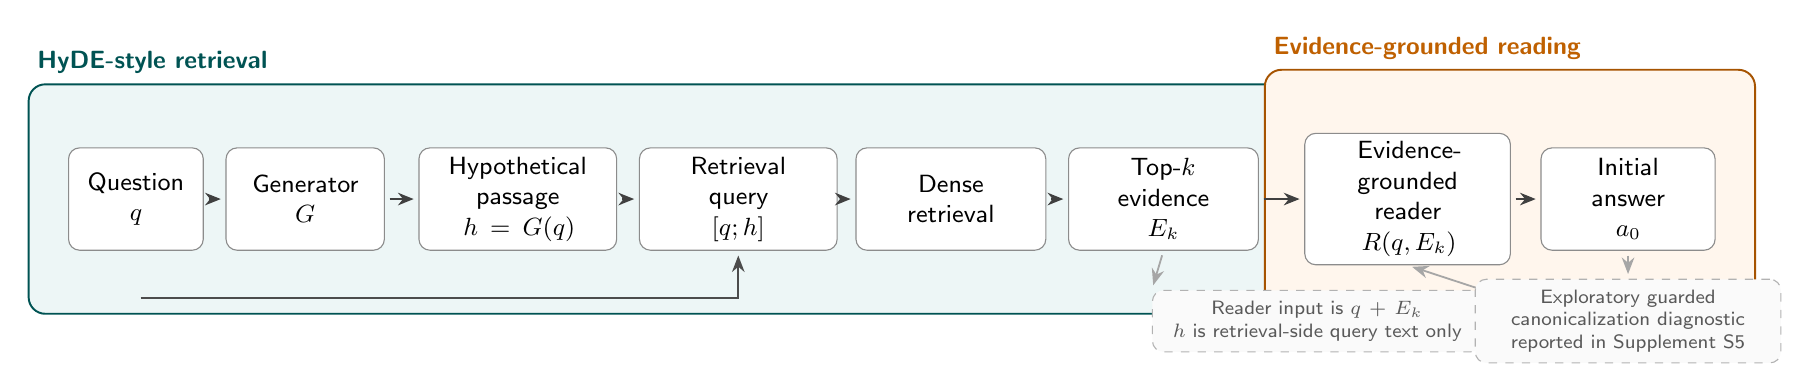
\begin{tikzpicture}[
    font=\sffamily\small,
    box/.style={draw=black!45, fill=white, rounded corners=4pt, align=center,
                minimum height=13mm, inner sep=3pt},
    arrow/.style={-{Stealth[length=2.1mm,width=1.6mm]}, draw=black!70, line width=0.65pt,
                  shorten <=0.6mm, shorten >=0.6mm},
    flowarrow/.style={-{Stealth[length=2.0mm,width=1.6mm]}, draw=black!75, line width=0.7pt,
                      shorten <=0.6mm, shorten >=0.6mm},
    stage/.style={draw=#1!65!black, fill=#1!7, rounded corners=6pt, line width=0.7pt},
    note/.style={draw=black!30, fill=gray!4, dashed, rounded corners=4pt,
                 align=center, font=\sffamily\scriptsize, text=black!65, inner sep=4pt}
]

\node[box, text width=15mm] (q) at (0,0) {Question\\$q$};
\node[box, text width=18mm] (gen) at (2.15,0) {Generator\\$G$};
\node[box, text width=23mm] (hyp) at (4.85,0) {Hypothetical\\passage\\$h=G(q)$};
\node[box, text width=23mm] (query) at (7.65,0) {Retrieval\\query\\$[q;h]$};
\node[box, text width=22mm] (retr) at (10.35,0) {Dense\\retrieval};
\node[box, text width=22mm] (evid) at (13.05,0) {Top-$k$\\evidence\\$E_k$};
\node[box, text width=24mm] (reader) at (16.15,0) {Evidence-grounded\\reader\\$R(q,E_k)$};
\node[box, text width=20mm] (ans) at (18.95,0) {Initial\\answer\\$a_0$};

\draw[flowarrow] (q.east) -- (gen.west);
\draw[flowarrow] (gen.east) -- (hyp.west);
\draw[flowarrow] (hyp.east) -- (query.west);
\draw[flowarrow] (query.east) -- (retr.west);
\draw[flowarrow] (retr.east) -- (evid.west);
\draw[flowarrow] (evid.east) -- (reader.west);
\draw[flowarrow] (reader.east) -- (ans.west);
\draw[arrow] ([yshift=-6mm]q.south) -| (query.south);

\node[note, text width=39mm] (boundary) at (15.0,-1.55)
{Reader input is $q+E_k$\\$h$ is retrieval-side query text only};
\draw[arrow, draw=black!35] (evid.south) -- (boundary.north west);
\draw[arrow, draw=black!35] (boundary.north east) -- (reader.south);

\node[note, text width=36mm] (diag) at (18.95,-1.55)
{Exploratory guarded\\canonicalization diagnostic\\reported in Supplement S5};
\draw[arrow, dashed, draw=black!35] (ans.south) -- (diag.north);

\begin{scope}[on background layer]
    \node[stage=teal, fit=(q)(gen)(hyp)(query)(retr)(evid), inner xsep=5mm, inner ysep=8mm] (stageRetrieval) {};
    \node[stage=orange, fit=(reader)(ans), inner xsep=5mm, inner ysep=8mm] (stageReader) {};
\end{scope}
\node[anchor=south west, font=\sffamily\bfseries\small, text=teal!65!black]
    at (stageRetrieval.north west) {HyDE-style retrieval};
\node[anchor=south west, font=\sffamily\bfseries\small, text=orange!75!black]
    at (stageReader.north west) {Evidence-grounded reading};

\end{tikzpicture}%
}
\caption{HyDE-style multi-hop RAG pipeline. The generated hypothetical passage is concatenated with the question for dense retrieval only; the reader receives the original question and retrieved corpus evidence. Guarded canonicalization is shown only as a small exploratory post-processing diagnostic and is detailed in the supplement.}
\label{fig:method_pipeline}
\end{figure*}

\section{Method}
\label{sec:method}

\subsection{Overview}
\label{sec:method_overview}

Under the evaluated protocol, multi-hop question answering is treated as evidence-grounded retrieval followed by reading. Given a question, the studied pipeline generates a concise hypothetical supporting passage, retrieves evidence with the question plus this passage, and asks an evidence-grounded short-answer LLM reader to produce an answer. Figure~\ref{fig:method_pipeline} summarizes the protocol, and Figure~\ref{fig:hyde_mechanism_overlap} summarizes the query-composition variants used in the diagnostic analysis.

The studied design centers on evidence acquisition rather than answer correction. HyDE-style retrieval targets supporting-title completeness before answer generation, with an artifact-level supporting-paragraph audit used to test whether title hits correspond to the processed gold paragraph texts. We additionally include a small exploratory guarded canonicalization diagnostic for answer-format risk cases; its selector, guards, and transition counts are reported in the supplement rather than treated as part of the primary method.

\subsection{Formal Protocol and Boundaries}
\label{sec:formal_protocol}

The primary retrieval-reader protocol takes as input a question $q$, a candidate corpus $\mathcal{C}=\{d_i\}_{i=1}^{N}$, and a retrieval budget $k$. Each document $d_i$ contains a title and paragraph text. The protocol returns an initial evidence-grounded short answer $a_0$ from retrieved corpus evidence.

\textbf{Primary retrieval-reader protocol.} A query-side generator $G$ maps the question to a hypothetical passage $h=G(q)$. The primary HyDE-style row uses the fixed dense retrieval query composition $[q;h]$; the question-only, rewritten-query, question-plus-rewritten-query, and hypothetical-only variants are query-composition diagnostic inputs rather than alternate final protocols. The primary inference rule is
\[
\begin{array}{l}
h=G(q),\\[2pt]
E_k=\mathrm{TopK}_{d\in\mathcal{C}}\,\mathrm{sim}(f([q;h]),f(d)),\\[2pt]
a_0=R(q,E_k).
\end{array}
\]

This protocol makes the reader-only evidence boundary explicit: the final reader never receives the hypothetical passage $h$ as evidence; it sees only $E_k$.

\subsection{Hypothetical Document Generation}
\label{sec:hypothetical_document_generation}

The hypothetical document generation module converts the original question into a retrieval-oriented passage. For each question, the LLM is prompted to write a concise passage that could contain the facts needed to answer the question. Its role is to provide a richer semantic query for retrieval.

This module targets multi-hop questions whose lexical cues can be sparse or indirect. A single question embedding may retrieve one supporting page while missing the second hop, especially when the second entity is only implied by the first piece of evidence. The hypothetical passage can make likely relations, entities, and answer types more explicit, giving dense retrieval a broader semantic target without requiring gold supporting facts.

\subsection{HyDE-Style Dense Retrieval}
\label{sec:hyde_retrieval}

HyDE-style retrieval uses the original question and the hypothetical passage as a combined dense query. In the main protocol, we first build a paragraph-level dense index over the local candidate corpus. Each document is represented by the concatenation of its title and paragraph text, encoded with the Sentence-Transformers implementation family introduced by Sentence-BERT \cite{reimers2019sentencebert}, using the \texttt{all-MiniLM-L6-v2} MiniLM-based encoder \cite{wang2020minilm}. The resulting embeddings are normalized and stored in a FAISS inner-product index \cite{johnson2019billion}. Because embeddings are normalized, inner-product search corresponds to cosine-style nearest-neighbour retrieval. BGE-base is used in the post-hoc stronger-encoder, equal-budget, corpus-scale, and hard-negative robustness diagnostics, without changing the primary MiniLM protocol or the reader prompts.

For each question, we concatenate the question with the generated hypothetical passage and encode the combined text with the same encoder. The resulting query embedding is searched against the dense index, and the top-$k$ documents are retained as the evidence set for the reader. The generated hypothetical passage is capped at 900 characters before query serialization, and all dense query-composition variants share the same MiniLM tokenizer and 256-token right-truncation policy documented in Supplement Section~\ref{supp:sec:supp_dense_encoder_truncation}.

The technical motivation for this module is that it targets supporting-evidence acquisition while preserving a bounded pipeline. Unlike full reasoning-trace retrieval, it does not require multi-step chain-of-thought generation or an open-ended planning agent. Unlike post-hoc verification, it acts before answer generation, where missing supporting pages or paragraphs can still be addressed by retrieving more complete context. The experiments therefore treat supporting-title completeness as the main diagnostic for whether the retrieval module works, and audit the same retrieval outputs at the normalized title--paragraph-text level where processed support flags are available.

\subsection{Evidence-Grounded Short-Answer LLM Reader}
\label{sec:short_answer_reader}

The evidence-grounded short-answer LLM reader converts the retrieved evidence set into a short factual answer. For each question, we serialize the top retrieved documents as ranked evidence blocks containing the document title and paragraph text. Each paragraph is truncated to a fixed character budget to keep the prompt compact while preserving the local context needed for answer generation.

The reader prompt instructs the model to use only the provided evidence, combine facts across evidence items when needed, and return only the exact short answer phrase requested by the question. The answer is not required to be a contiguous span copied from a single evidence passage: the reader may combine evidence items and perform simple date, age, comparison, or yes/no reasoning, while being explicitly instructed not to rely on information outside the retrieved evidence. The prompt also includes generic short-answer formatting instructions derived from common multi-hop QA answer types, including yes/no questions, location questions, date or age comparisons, and role or position questions. These generic formatting instructions were fixed before the canonical evaluation pass and applied unchanged to HotpotQA and 2WikiMultihopQA. They are intended to reduce answer-format drift without giving the reader access to gold answers or evaluation labels. In the main experiments, the reader is called through an OpenAI-compatible API interface with temperature-0 decoding.

\subsection{Implementation Details}
\label{sec:implementation_boundary}

All generation modules use fixed prompt templates. The HyDE prompt asks for one concise hypothetical supporting passage, and the reader prompt asks for an exact short answer from retrieved evidence only. The generation wrapper calls Qwen3.7-Max through an OpenAI-compatible API interface with \texttt{temperature=0.0}. The reported \texttt{max\_tokens} settings are 64 for HyDE passage generation, 64 for rewritten-query generation, and 64 for reader answers. The prompt JSONL artifacts retain gold-answer metadata for evaluation and auditing, but the gold answer is not inserted into the prompt text shown to the model.

% Figure 2 uses the externally supplied SVG/PDF artwork.
% Required packages:
% \usepackage{tikz}
% \usetikzlibrary{arrows.meta,positioning,fit,backgrounds}
% \usepackage{xcolor}
% \usepackage{graphicx}

\begin{figure*}[t]
\centering
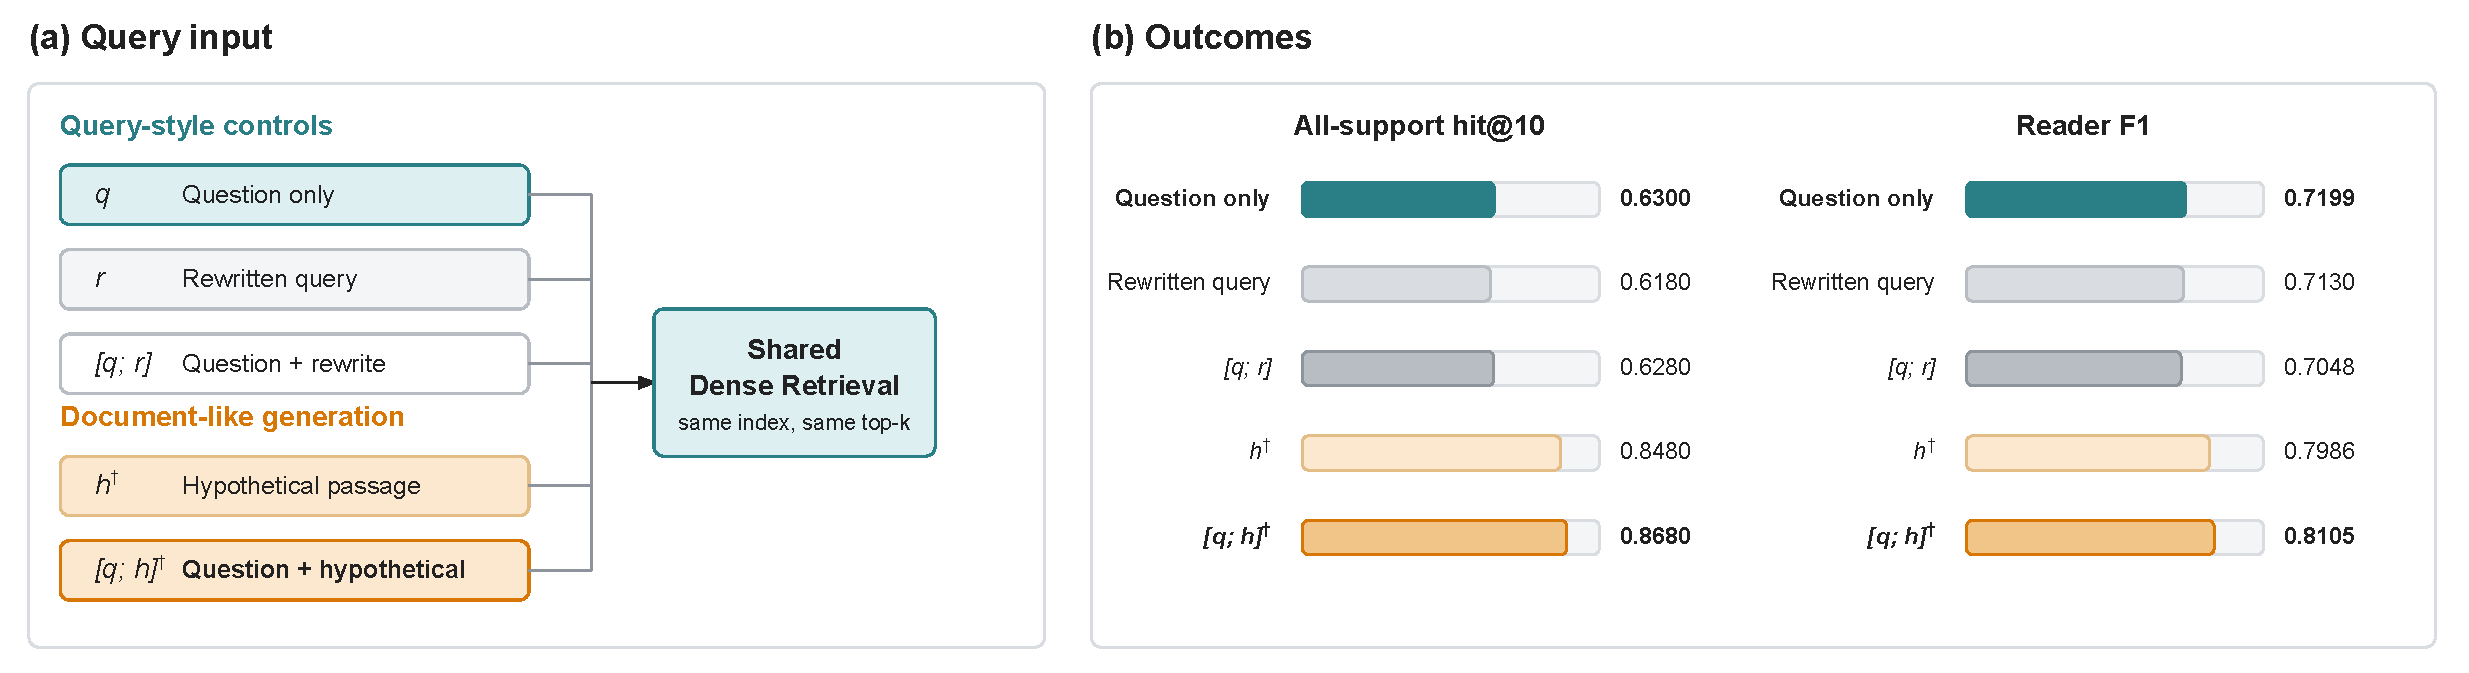
\includegraphics[width=\textwidth]{../figures/figure2.pdf}
\iffalse
\resizebox{\textwidth}{!}{%
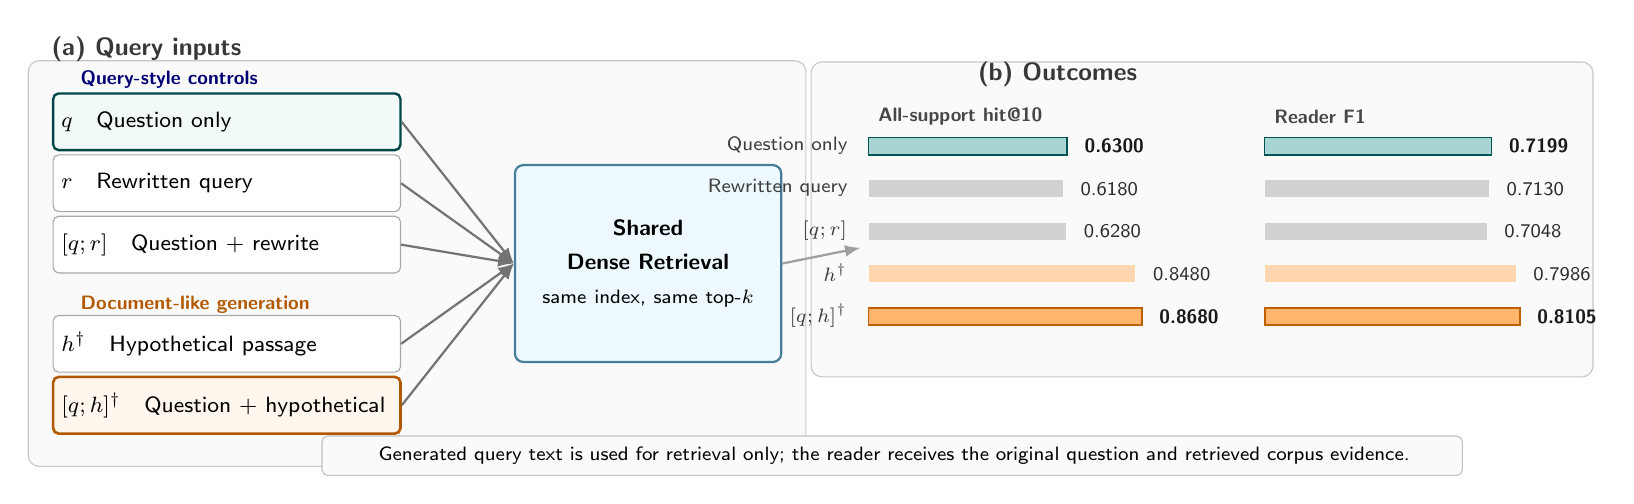
\begin{tikzpicture}[
    font=\sffamily\footnotesize,
    input/.style={draw=black!34, rounded corners=2pt, fill=white, align=left,
                  text width=42mm, minimum height=7.2mm, inner sep=3pt},
    inputemph/.style={input, draw=teal!55!black, line width=0.85pt, fill=teal!5},
    inputhyde/.style={input, draw=orange!70!black, line width=0.95pt, fill=orange!7},
    retr/.style={draw=cyan!55!black, rounded corners=3pt, fill=cyan!7, align=center,
                 text width=31mm, minimum height=25mm, inner sep=4pt, line width=0.8pt},
    group/.style={draw=black!22, rounded corners=4pt, fill=black!2, inner xsep=3mm, inner ysep=4mm},
    qgroup/.style={draw=blue!40!black, rounded corners=4pt, fill=blue!4, inner xsep=2.5mm, inner ysep=4mm},
    hgroup/.style={draw=orange!65!black, rounded corners=4pt, fill=orange!5, inner xsep=2.5mm, inner ysep=4mm},
    panel/.style={font=\sffamily\bfseries\small, text=black!78},
    axislabel/.style={font=\sffamily\bfseries\scriptsize, text=black!72},
    barlabel/.style={font=\sffamily\scriptsize, text=black!76, align=right},
    value/.style={font=\sffamily\scriptsize, text=black!82},
    valueemph/.style={font=\sffamily\bfseries\scriptsize, text=black!90},
    arrow/.style={-{Latex[length=2.0mm]}, thick, draw=black!55},
    softarrow/.style={-{Latex[length=2.0mm]}, thick, draw=black!38}
]

% Panel (a): query inputs and shared retrieval.
\node[panel, anchor=west] at (-2.35,0.74) {(a) Query inputs};
\node[font=\sffamily\bfseries\scriptsize, text=blue!45!black, anchor=west] at (-1.98,0.36) {Query-style controls};
\node[inputemph] (q) at (0,-0.18) {\textbf{$q$}\quad Question only};
\node[input] (r) at (0,-0.96) {\textbf{$r$}\quad Rewritten query};
\node[input] (qr) at (0,-1.74) {\textbf{$[q;r]$}\quad Question + rewrite};
\node[font=\sffamily\bfseries\scriptsize, text=orange!70!black, anchor=west] at (-1.98,-2.50) {Document-like generation};
\node[input] (h) at (0,-3.00) {\textbf{$h^\dagger$}\quad Hypothetical passage};
\node[inputhyde] (qh) at (0,-3.78) {\textbf{$[q;h]^\dagger$}\quad Question + hypothetical};

\node[retr] (retrieval) at (5.35,-1.98) {\textbf{Shared}\\[1mm]\textbf{Dense Retrieval}\\[1mm]\scriptsize same index, same top-$k$};

\draw[arrow] (q.east) -- (retrieval.west);
\draw[arrow] (r.east) -- (retrieval.west);
\draw[arrow] (qr.east) -- (retrieval.west);
\draw[arrow] (h.east) -- (retrieval.west);
\draw[arrow] (qh.east) -- (retrieval.west);

\begin{scope}[on background layer]
    \node[qgroup, fit=(q)(r)(qr)] {};
    \node[hgroup, fit=(h)(qh)] {};
    \node[group, fit=(q)(r)(qr)(h)(qh)(retrieval)] {};
\end{scope}

% Panel (b): compact result bars.
\node[panel] at (10.55,0.42) {(b) Outcomes};
\node[axislabel, anchor=west] at (8.15,-0.12) {All-support hit@10};
\node[axislabel, anchor=west] at (13.18,-0.12) {Reader F1};

\node[barlabel, anchor=east, text width=21mm] at (8.0,-0.48) {Question only};
\node[barlabel, anchor=east, text width=21mm] at (8.0,-1.02) {Rewritten query};
\node[barlabel, anchor=east, text width=21mm] at (8.0,-1.56) {$[q;r]$};
\node[barlabel, anchor=east, text width=21mm] at (8.0,-2.10) {$h^\dagger$};
\node[barlabel, anchor=east, text width=21mm] at (8.0,-2.64) {$[q;h]^\dagger$};

% All-support hit@10 bars.
\fill[teal!34] (8.15,-0.60) rectangle ++(2.52,0.22);
\draw[teal!65!black, line width=0.55pt] (8.15,-0.60) rectangle ++(2.52,0.22);
\node[valueemph, anchor=west] at (10.77,-0.49) {0.6300};
\fill[black!18] (8.15,-1.14) rectangle ++(2.47,0.22);
\node[value, anchor=west] at (10.72,-1.03) {0.6180};
\fill[black!18] (8.15,-1.68) rectangle ++(2.51,0.22);
\node[value, anchor=west] at (10.76,-1.57) {0.6280};
\fill[orange!32] (8.15,-2.22) rectangle ++(3.39,0.22);
\node[value, anchor=west] at (11.64,-2.11) {0.8480};
\fill[orange!58] (8.15,-2.76) rectangle ++(3.47,0.22);
\draw[orange!75!black, line width=0.65pt] (8.15,-2.76) rectangle ++(3.47,0.22);
\node[valueemph, anchor=west] at (11.72,-2.65) {0.8680};

% Reader F1 bars.
\fill[teal!34] (13.18,-0.60) rectangle ++(2.88,0.22);
\draw[teal!65!black, line width=0.55pt] (13.18,-0.60) rectangle ++(2.88,0.22);
\node[valueemph, anchor=west] at (16.16,-0.49) {0.7199};
\fill[black!18] (13.18,-1.14) rectangle ++(2.85,0.22);
\node[value, anchor=west] at (16.13,-1.03) {0.7130};
\fill[black!18] (13.18,-1.68) rectangle ++(2.82,0.22);
\node[value, anchor=west] at (16.10,-1.57) {0.7048};
\fill[orange!32] (13.18,-2.22) rectangle ++(3.19,0.22);
\node[value, anchor=west] at (16.47,-2.11) {0.7986};
\fill[orange!58] (13.18,-2.76) rectangle ++(3.24,0.22);
\draw[orange!75!black, line width=0.65pt] (13.18,-2.76) rectangle ++(3.24,0.22);
\node[valueemph, anchor=west] at (16.52,-2.65) {0.8105};

\draw[softarrow] (retrieval.east) -- (8.05,-1.78);

\begin{scope}[on background layer]
    \node[group, fit={(7.72,-3.02)(17.05,0.18)}] {};
\end{scope}

\node[draw=black!24, rounded corners=2pt, fill=black!2, align=center,
      text width=142mm, inner sep=4pt, font=\sffamily\scriptsize]
      at (8.45,-4.42)
      {Generated query text is used for retrieval only; the reader receives the original question and retrieved corpus evidence.};

\end{tikzpicture}%
}
\fi
\caption{HyDE query-composition diagnostic. Panel (a) groups query-style controls ($q$, $r$, and $[q;r]$) and document-like generation ($h$ and $[q;h]$), all passed to the same dense retrieval stage. Panel (b) reports HotpotQA all-support hit@10 and reader F1 for the same five inputs, with question only and question + hypothetical passage visually emphasized. The dagger ($^\dagger$) marks generated hypothetical text covered by the answer-string-overlap diagnostic.}
\label{fig:hyde_mechanism_overlap}
\end{figure*}

% Compact main-paper tables for the HyDE-enhanced RAG manuscript.

\begin{table*}[t]
\centering
\caption{Main results on the released IRCoT HotpotQA \texttt{test\_subsampled} split.}
\label{tab:main_results}
\scriptsize
\begin{threeparttable}
\setlength{\tabcolsep}{3pt}
\begin{tabularx}{\textwidth}{>{\raggedright\arraybackslash}X r r r r r}
\toprule
Method & Any hit@10 & All hit@10 & Recall@10 & EM & F1 \\
\midrule
LLM-only / No Retrieval & -- & -- & -- & 0.5200 & 0.6658 \\
One-step Dense RAG & 0.9860 & 0.6300 & 0.8080 & 0.5940 & 0.7199 \\
Multi-query RAG & 0.9860 & 0.6300 & 0.8080 & 0.5860 & 0.7028 \\
Single-query Reformulation RAG & 0.9800 & 0.6180 & 0.7990 & 0.5960 & 0.7130 \\
BM25 RAG & 0.9860 & 0.7320 & 0.8590 & 0.6240 & 0.7436 \\
BM25 + Dense Hybrid & \best{0.9900} & 0.7480 & 0.8690 & 0.6400 & 0.7577 \\
Rule-based Evidence-Expanded Iterative Retrieval & 0.9860 & 0.7540 & 0.8700 & 0.6360 & 0.7565 \\
\rowcolor{gray!10} HyDE-style RAG & 0.9880 & \best{0.8680} & \best{0.9280} & \best{0.6840} & \best{0.8105} \\
\bottomrule
\end{tabularx}
\begin{tablenotes}
\footnotesize
\item Bold marks column maxima; the shaded row marks the primary HyDE-style retrieval-reader method. All rows are evaluated on 500 HotpotQA examples with the hosted API model string \texttt{qwen3.7-max} as the reader. Retrieval rows use top-$k=10$ evidence; the LLM-only row has no retrieval. This setting uses the processed local-corpus protocol and should not be described as a full reproduction of the original full-wiki IRCoT setup. Dense, BM25, and Hybrid are implemented lightweight retrieval baselines; Single-query Reformulation RAG is a matched-call mechanism control; Multi-query RAG and Rule-based Evidence-Expanded Iterative Retrieval are fixed heuristic controls rather than faithful reproductions of published multi-query or IRCoT-style systems. The Multi-query row has the same supporting-title hit metrics as one-step Dense RAG because it retrieves the same top-10 document sets under the selected rule-based query variants, although the ranking order changes. The small guarded canonicalization diagnostic is reported in Supplement Section~\ref{supp:sec:supp_verifier_guard_decomposition} rather than as a primary result row.
\end{tablenotes}
\end{threeparttable}
\end{table*}

\begin{table*}[t]
\centering
\caption{HyDE query-composition diagnostic on the released IRCoT HotpotQA \texttt{test\_subsampled} split.}
\label{tab:hyde_query_ablation}
\small
\begin{threeparttable}
\begin{tabularx}{\textwidth}{>{\raggedright\arraybackslash}X r r r r r}
\toprule
Query used for dense retrieval & Any hit@10 & All hit@10 & Recall@10 & EM & F1 \\
\midrule
Question only & 0.9860 & 0.6300 & 0.8080 & 0.5940 & 0.7199 \\
Single rewritten query & 0.9800 & 0.6180 & 0.7990 & 0.5960 & 0.7130 \\
Question + rewritten query & 0.9780 & 0.6280 & 0.8030 & 0.5800 & 0.7048 \\
Hypothetical passage only & \best{0.9880} & 0.8480 & 0.9180 & 0.6780 & 0.7986 \\
Question + hypothetical passage & \best{0.9880} & \best{0.8680} & \best{0.9280} & \best{0.6840} & \best{0.8105} \\
\bottomrule
\end{tabularx}
\begin{tablenotes}
\footnotesize
\item All rows use the same MiniLM dense index, top-$k=10$, evidence-grounded short-answer reader prompt, and Qwen3.7-Max reader. Query serialization and MiniLM tokenization/truncation are shared across the question-only, single rewritten query, question + rewritten query, hypothetical-only, and question + hypothetical rows; the exact dense encoder configuration is reported in Supplement Section~\ref{supp:sec:supp_dense_encoder_truncation}. The question-only row reproduces the one-step dense retrieval baseline. The single rewritten query row uses one additional Qwen3.7-Max call to generate a concise retrieval query, matching the query-side call budget of HyDE without generating a document-like hypothetical passage. The question + rewritten query row additionally tests whether the observed HyDE advantage is explained by retaining the original question in the dense query. The hypothetical-only row uses the generated passage only as the retrieval query; the reader receives only retrieved evidence passages.
\end{tablenotes}
\end{threeparttable}
\end{table*}

\begin{table*}[t]
\centering
\caption{Secondary generalization check on the released IRCoT 2WikiMultihopQA \texttt{test\_subsampled} split.}
\label{tab:2wiki_generalization}
\small
\begin{threeparttable}
\begin{tabularx}{\textwidth}{>{\raggedright\arraybackslash}X r r r r r}
\toprule
Method & Any hit@10 & All hit@10 & Recall@10 & EM & F1 \\
\midrule
One-step Dense RAG & 0.9840 & 0.3580 & 0.6695 & 0.5400 & 0.5767 \\
BM25 RAG & \best{0.9980} & 0.4320 & 0.7250 & 0.5840 & 0.6169 \\
BM25 + Dense Hybrid & \best{0.9980} & 0.4480 & 0.7330 & 0.5840 & 0.6220 \\
HyDE-style RAG & 0.9940 & \best{0.6680} & \best{0.8575} & \best{0.6620} & \best{0.7289} \\
\bottomrule
\end{tabularx}
\begin{tablenotes}
\footnotesize
\item All methods use Qwen3.7-Max, $N=500$, and top-$k=10$. The 2WikiMultihopQA split is used as a secondary generalization check rather than as the main benchmark. All rows use the same processed local-corpus protocol and evidence-grounded short-answer reader prompt. BM25 and Hybrid tie on EM, but Hybrid obtains slightly higher token F1; both remain below HyDE-style RAG.
\end{tablenotes}
\end{threeparttable}
\end{table*}

\begin{table*}[t]
\centering
\caption{Stronger dense-encoder query-composition robustness check with \texttt{BAAI/bge-base-en-v1.5}.}
\label{tab:stronger_encoder_reproduction}
\scriptsize
\begin{threeparttable}
\setlength{\tabcolsep}{3pt}
\begin{tabularx}{\textwidth}{l >{\raggedright\arraybackslash}X r r r r r}
\toprule
Dataset & Query used for dense retrieval & Any hit@10 & All hit@10 & Recall@10 & EM & F1 \\
\midrule
HotpotQA & Question only & \best{0.9940} & 0.8820 & 0.9380 & 0.6840 & 0.8153 \\
HotpotQA & Single rewritten query & 0.9920 & 0.8340 & 0.9130 & 0.6680 & 0.7965 \\
HotpotQA & Question + rewritten query & \best{0.9940} & 0.8520 & 0.9230 & 0.6760 & 0.8055 \\
HotpotQA & Hypothetical passage only & 0.9900 & 0.9080 & 0.9490 & \best{0.7040} & \best{0.8274} \\
\rowcolor{gray!10} HotpotQA & Question + hypothetical passage & \best{0.9940} & \best{0.9200} & \best{0.9570} & 0.7020 & 0.8267 \\
\midrule
2Wiki & Question only & 0.9980 & 0.5100 & 0.7655 & 0.6160 & 0.6609 \\
2Wiki & Single rewritten query & \best{1.0000} & 0.4720 & 0.7380 & 0.5840 & 0.6291 \\
2Wiki & Question + rewritten query & 0.9940 & 0.4540 & 0.7320 & 0.5940 & 0.6366 \\
2Wiki & Hypothetical passage only & \best{1.0000} & \best{0.8220} & \best{0.9275} & \best{0.6780} & \best{0.7459} \\
\rowcolor{gray!10} 2Wiki & Question + hypothetical passage & \best{1.0000} & 0.7800 & 0.9130 & 0.6740 & 0.7343 \\
\bottomrule
\end{tabularx}
\begin{tablenotes}
\footnotesize
\item All rows use the stronger BGE-base encoder, top-$k=10$, the same processed local-corpus protocol, and the same Qwen3.7-Max reader. Bold marks the best value within each dataset block; shaded rows mark the primary HyDE-style query serialization used in the main MiniLM pipeline. This table tests whether the query-composition pattern persists beyond the MiniLM dense encoder; it is not a tuned replacement for the main retrieval-reader system.
\end{tablenotes}
\end{threeparttable}
\end{table*}

\begin{table*}[t]
\centering
\caption{Strict equal-budget retrieval-only query-form diagnostic and paired contrasts with \texttt{BAAI/bge-base-en-v1.5}.}
\label{tab:equal_budget_retrieval_diagnostic}
\scriptsize
\begin{threeparttable}
\setlength{\tabcolsep}{3pt}
\begin{tabularx}{\textwidth}{l >{\raggedright\arraybackslash}X r r r r}
\toprule
Dataset & Generated query form & Mean words & Any hit@10 & All hit@10 & Recall@10 \\
\midrule
HotpotQA & Keyword/entity expansion & 38.370 & 0.9900 & 0.9240 & 0.9570 \\
HotpotQA & Direct rewrite & 39.392 & 0.9860 & 0.8800 & 0.9330 \\
HotpotQA & Question decomposition & 39.640 & 0.9900 & 0.8740 & 0.9320 \\
\rowcolor{gray!10} HotpotQA & Document-like passage & 39.246 & \best{0.9940} & \best{0.9260} & \best{0.9600} \\
\midrule
2Wiki & Keyword/entity expansion & 38.170 & 0.9920 & 0.6760 & 0.8410 \\
2Wiki & Direct rewrite & 39.628 & 0.9680 & 0.4760 & 0.7190 \\
2Wiki & Question decomposition & 40.008 & 0.9980 & 0.4540 & 0.7295 \\
\rowcolor{gray!10} 2Wiki & Document-like passage & 39.172 & \best{1.0000} & \best{0.7520} & \best{0.9035} \\
\bottomrule
\end{tabularx}
\medskip
\begin{tabularx}{\textwidth}{l >{\raggedright\arraybackslash}X r r r}
\toprule
Dataset & Baseline form & $N$ & $\Delta$ All hit@10 [95\% CI] & $\Delta$ Recall@10 [95\% CI] \\
\midrule
HotpotQA & Direct rewrite & 500 & +0.0460 [+0.0200, +0.0720] & +0.0270 [+0.0120, +0.0410] \\
HotpotQA & Question decomposition & 500 & +0.0520 [+0.0260, +0.0800] & +0.0280 [+0.0140, +0.0430] \\
HotpotQA & Keyword/entity expansion & 500 & +0.0020 [-0.0180, +0.0220] & +0.0030 [-0.0080, +0.0140] \\
\midrule
2Wiki & Direct rewrite & 500 & +0.2760 [+0.2360, +0.3160] & +0.1845 [+0.1620, +0.2070] \\
2Wiki & Question decomposition & 500 & +0.2980 [+0.2580, +0.3420] & +0.1740 [+0.1530, +0.1940] \\
2Wiki & Keyword/entity expansion & 500 & +0.0760 [+0.0440, +0.1080] & +0.0625 [+0.0460, +0.0800] \\
\bottomrule
\end{tabularx}
\begin{tablenotes}
\footnotesize
\item Each row evaluates 500 examples. All forms use the same Qwen3.7-Max generator, one generation call per question, a 40-word target with a shared 64-token generation cap, the same BGE-base encoder, query serialization and encoder truncation, and top-$k=10$. Retrieval encodes the original question plus the generated text, serialized as \texttt{question}, the label \texttt{Generated retrieval text:}, and the generated output; the document-like row is therefore $[q;G_{\mathrm{doc}}(q)]$, not $G_{\mathrm{doc}}(q)$ alone. The table is retrieval-only: reader answers are not regenerated. Bold marks the largest point estimate in each dataset block; shaded rows mark the document-like form. The lower panel reports document-like passage minus the named baseline using question-level paired bootstrap 95\% percentile intervals ($B=2000$, seed 13). Realized mean length ranges from 38.170 to 40.008 words.
\end{tablenotes}
\end{threeparttable}
\end{table*}

\begin{table*}[t]
\centering
\caption{Targeted Qwen-Turbo reader paired check on fixed equal-budget evidence.}
\label{tab:equal_budget_reader_check}
\scriptsize
\begin{threeparttable}
\setlength{\tabcolsep}{3pt}
\begin{tabularx}{\textwidth}{lXrrrrcc}
\toprule
Dataset & Baseline $\rightarrow$ doc-like & Baseline EM/F1 & Doc-like EM/F1 & $\Delta$EM & $\Delta$F1 [95\% CI] & W$\rightarrow$C / C$\rightarrow$W & McNemar $p$ \\
\midrule
HotpotQA & Direct rewrite $\rightarrow$ doc-like & 0.4960/0.6294 & 0.5660/0.7046 & 0.0700 & 0.0752 [0.0495, 0.1001] & 45 / 10 & $<0.0001$ \\
HotpotQA & Keyword/entity expansion $\rightarrow$ doc-like & 0.5500/0.6777 & 0.5660/0.7046 & 0.0160 & 0.0269 [0.0053, 0.0503] & 24 / 16 & 0.2682 \\
2Wiki & Direct rewrite $\rightarrow$ doc-like & 0.3460/0.4148 & 0.3620/0.4498 & 0.0160 & 0.0350 [0.0006, 0.0727] & 48 / 40 & 0.4557 \\
2Wiki & Keyword/entity expansion $\rightarrow$ doc-like & 0.3640/0.4498 & 0.3620/0.4498 & -0.0020 & 0.0000 [-0.0354, 0.0342] & 36 / 37 & 1.0000 \\
\bottomrule
\end{tabularx}
\begin{tablenotes}
\footnotesize
\item All rows reuse the fixed top-10 evidence from the strict equal-budget BGE-base retrieval diagnostic and regenerate only reader answers with \texttt{qwen-turbo}. $\Delta$ values are document-like passage minus the named baseline over 500 paired examples. F1 intervals are paired bootstrap 95\% confidence intervals. W$\rightarrow$C and C$\rightarrow$W are EM transitions for document-like versus the baseline; McNemar's exact test is computed on these discordant EM counts.
\end{tablenotes}
\end{threeparttable}
\end{table*}

\begin{table*}[t]
\centering
\caption{Corpus-scale retrieval stress test with processed-train distractor expansion. The Local rows reuse the retained-duplicate BGE local-index artifacts from Table~\ref{tab:stronger_encoder_reproduction}; only the 50k and 100k rows use newly expanded stress-test corpora.}
\label{tab:corpus_scale_stress}
\scriptsize
\begin{threeparttable}
\setlength{\tabcolsep}{3pt}
\begin{tabularx}{\textwidth}{l r rr rr rr >{\raggedright\arraybackslash}X}
\toprule
Dataset & Docs & \multicolumn{2}{c}{Question only} & \multicolumn{2}{c}{Single rewrite} & \multicolumn{2}{c}{Question + hypothetical} & HyDE all-hit delta \\
\cmidrule(lr){3-4}\cmidrule(lr){5-6}\cmidrule(lr){7-8}
 & & All & Recall & All & Recall & All & Recall & vs. question; vs. single rewrite \\
\midrule
HotpotQA & Local & 0.8820 & 0.9380 & 0.8340 & 0.9130 & \best{0.9200} & \best{0.9570} & +0.0380 [0.0100, 0.0660]; +0.0860 [0.0560, 0.1160] \\
HotpotQA & 50k & 0.7480 & 0.8650 & 0.6520 & 0.8120 & \best{0.8560} & \best{0.9210} & +0.1080 [0.0680, 0.1460]; +0.2040 [0.1620, 0.2440] \\
HotpotQA & 100k & 0.6960 & 0.8380 & 0.5960 & 0.7820 & \best{0.8340} & \best{0.9060} & +0.1380 [0.1000, 0.1780]; +0.2380 [0.1940, 0.2800] \\
\midrule
2Wiki & Local & 0.5100 & 0.7655 & 0.4720 & 0.7380 & \best{0.7800} & \best{0.9130} & +0.2700 [0.2300, 0.3100]; +0.3080 [0.2680, 0.3520] \\
2Wiki & 50k & 0.4460 & 0.7270 & 0.4040 & 0.6900 & \best{0.6900} & \best{0.8655} & +0.2440 [0.2040, 0.2840]; +0.2860 [0.2440, 0.3280] \\
2Wiki & 100k & 0.4180 & 0.7105 & 0.3600 & 0.6620 & \best{0.6500} & \best{0.8440} & +0.2320 [0.1900, 0.2760]; +0.2900 [0.2460, 0.3340] \\
\bottomrule
\end{tabularx}
\begin{tablenotes}
\footnotesize
\item All rows use \texttt{BAAI/bge-base-en-v1.5}, top-$k=10$, and 500 examples. Single rewrite denotes the Single rewritten query condition from Table~\ref{tab:stronger_encoder_reproduction}, not the question-plus-rewritten-query composition or the equal-budget direct-rewrite diagnostic. Local denotes the original retained-duplicate local index used in Table~\ref{tab:stronger_encoder_reproduction} (4,977 HotpotQA documents and 5,000 2Wiki documents). The rounded 5k stress-test cache is not used as a Table~\ref{tab:stronger_encoder_reproduction} replicate because the stress-construction script exact-deduplicates title--paragraph records before expansion and, for HotpotQA, pads the 4,977-document local corpus to 5,000 with train distractors. The 50k and 100k corpora preserve the released evaluation corpus and add exact-title--paragraph-deduplicated processed-train distractor passages sampled with seed 20260721. This is a retrieval-only stress test, not a full-wiki experiment. Intervals are paired bootstrap 95\% confidence intervals over per-example all-support hit@10 deltas. Full any-hit, recall-delta, artifact-path, and construction details are reported in the supplemental corpus-scale stress-test table.
\end{tablenotes}
\end{threeparttable}
\end{table*}

\begin{table*}[t]
\centering
\caption{Corpus-scale leakage and BGE hard-negative audit.}
\label{tab:corpus_scale_audit}
\scriptsize
\begin{threeparttable}
\setlength{\tabcolsep}{3pt}
\begin{tabularx}{\textwidth}{llrrrrrrr}
\toprule
Dataset & Stress corpus & Docs & Gold-title add. & Near-dup gold & Sim p95 & Q All & HyDE All & $\Delta$All \\
\midrule
HotpotQA & Random 100k & 100000 & 1 & 1 & 0.6011 & 0.6960 & 0.8340 & 0.1380 \\
HotpotQA & No-gold-title 100k & 99999 & 0 & 0 & 0.6011 & 0.6960 & 0.8340 & 0.1380 \\
HotpotQA & BGE-hard 50k & 50000 & 0 & 0 & 0.6204 & 0.6960 & 0.8420 & 0.1460 \\
2WikiMultihopQA & Random 100k & 100000 & 173 & 173 & 0.5948 & 0.4180 & 0.6500 & 0.2320 \\
2WikiMultihopQA & No-gold-title 100k & 99827 & 0 & 0 & 0.5948 & 0.4180 & 0.6520 & 0.2340 \\
2WikiMultihopQA & BGE-hard 50k & 50000 & 0 & 0 & 0.6172 & 0.4180 & 0.6580 & 0.2400 \\
\bottomrule
\end{tabularx}
\begin{tablenotes}
\footnotesize
\item The random 100k rows audit the existing processed-train distractor expansion. The no-gold-title rows remove only added train records whose normalized title matches any test supporting title, while preserving the released evaluation corpus. The BGE-hard rows keep the released evaluation corpus and select the most question-similar added train distractors from the audited 100k pool after the same gold-title exclusion; they are a harder 50k diagnostic, not a larger index. Sim p95 is the 95th percentile of each added distractor's maximum BGE cosine similarity to any test question. Near-dup gold counts added records whose token-Jaccard similarity to any test gold supporting paragraph is at least 0.85.
\end{tablenotes}
\end{threeparttable}
\end{table*}

\begin{table*}[t]
\centering
\caption{Top-$k$ sensitivity and supporting-title rank audit for fixed-ranking retrieval variants.}
\label{tab:topk_sensitivity}
\scriptsize
\begin{threeparttable}
\setlength{\tabcolsep}{3pt}
\begin{tabularx}{\textwidth}{llrrrrrrrrr}
\toprule
Dataset & Method & All@5 & All@10 & All@20 & Rec@5 & Rec@10 & Rec@20 & Capped mean worst rank & Capped median worst rank & Miss@20 \\
\midrule
HotpotQA & Dense & 0.5060 & 0.6300 & 0.7240 & 0.7340 & 0.8080 & 0.8570 & 9.56 & 5.0 & 138 \\
HotpotQA & BM25 & 0.5080 & 0.7320 & 0.8520 & 0.7310 & 0.8590 & 0.9250 & 7.98 & 5.0 & 74 \\
HotpotQA & Direct rewrite & 0.4760 & 0.6180 & 0.7100 & 0.7160 & 0.7990 & 0.8480 & 9.90 & 6.0 & 145 \\
HotpotQA & HyDE & 0.7760 & 0.8680 & 0.9080 & 0.8800 & 0.9280 & 0.9510 & 5.20 & 2.0 & 46 \\
2WikiMultihopQA & Dense & 0.2740 & 0.3580 & 0.4220 & 0.6185 & 0.6695 & 0.7100 & 14.50 & 21.0 & 289 \\
2WikiMultihopQA & BM25 & 0.3300 & 0.4320 & 0.4740 & 0.6645 & 0.7250 & 0.7495 & 13.31 & 21.0 & 263 \\
2WikiMultihopQA & Direct rewrite & 0.2860 & 0.3680 & 0.4240 & 0.6335 & 0.6800 & 0.7140 & 14.35 & 21.0 & 288 \\
2WikiMultihopQA & HyDE & 0.5880 & 0.6680 & 0.7140 & 0.8085 & 0.8575 & 0.8825 & 8.81 & 4.0 & 143 \\
\bottomrule
\end{tabularx}
\begin{tablenotes}
\footnotesize
\item All rows are rescored from top-20 retrieval artifacts generated from frozen questions and frozen generated query text; no new LLM calls are used. The depth-sensitive RRF fusion control is omitted because changing the per-branch candidate depth for top-20 fusion changes the fused top-10 ranking relative to the canonical fusion rows in Tables~\ref{tab:main_results} and~\ref{tab:2wiki_generalization}. All@k requires all annotated supporting titles to appear within the first k retrieved documents. Rec@k is mean supporting-title recall at k. Capped worst-rank columns use the worst supporting-title rank per question, with supports not retrieved in the top 20 capped at 21; Miss@20 counts examples with at least one supporting title still absent by rank 20.
\end{tablenotes}
\end{threeparttable}
\end{table*}

\section{Experiments}
\label{sec:experiments}

\subsection{Protocol}
\label{sec:dataset_setting}

We evaluate the studied HyDE-style pipeline on released IRCoT processed multi-hop QA splits under a processed local-corpus protocol. HotpotQA \texttt{test\_subsampled} is the main benchmark, and 2WikiMultihopQA \texttt{test\_subsampled} is used as a secondary generalization check. Each split contains 500 examples with supporting-title annotations and a local candidate evidence pool; corpus statistics and artifact provenance are reported in the supplement. The corpus is indexed jointly within each dataset, but the candidate paragraphs are question-tagged artifacts from the released processed data rather than a full Wikipedia collection. This setting enables paired comparison across retrieval variants on identical examples and evidence pools, but it is not a full-wiki reproduction of the original IRCoT retrieval setting.

All retrieval-reader systems use top-$k=10$ evidence passages and the same evidence-grounded short-answer reader prompt. Retrieval quality is measured by any supporting-title hit@10, all supporting-title hit@10, and mean supporting-title recall@10; answer quality is measured by normalized Exact Match (EM) and token-level F1. Because the jointly indexed corpus is constructed from released question-level candidate pools that already contain annotated support passages and semantically related distractors, we emphasize all-support hit@10 and supporting-title recall@10 over any-hit@10. The corpus records also retain \texttt{is\_supporting} flags, so Supplement Section~\ref{supp:sec:supp_evidence_case_artifacts} and Supplement Table~\ref{supp:tab:supporting_paragraph_audit} audit the same retrieval files with exact normalized title--paragraph-text matching. In the released processed splits, each annotated supporting title is associated with one supporting paragraph record, so the paragraph audit primarily verifies exact processed-record recovery rather than introducing an independent sentence-level evidence notion. This audit gives the same all-support and recall values as the title-level metrics for the audited rows listed in Supplement Table~\ref{supp:tab:supporting_paragraph_audit}, while the 500-example JSONL artifacts do not expose gold supporting sentence text for sentence-level fact coverage. The main HotpotQA table uses a MiniLM dense stack: the Sentence-Transformers implementation family introduced by Sentence-BERT \cite{reimers2019sentencebert}, the \texttt{all-MiniLM-L6-v2} MiniLM-based encoder \cite{wang2020minilm}, and a FAISS inner-product index over normalized paragraph embeddings \cite{johnson2019billion}. The BGE-base experiments are reported as stronger-encoder robustness checks rather than as a tuned replacement for the main protocol: we rerun the query-composition variants with \texttt{BAAI/bge-base-en-v1.5} \cite{xiao2023cpack} without changing prompts, top-$k$, reader settings, or the processed local-corpus protocol. Only document titles and paragraph texts are encoded for retrieval; question identifiers, supporting-evidence flags, gold answers, and evaluation metadata are excluded from retrieval representations. Qwen3.7-Max is used through an OpenAI-compatible chat-completions interface for query generation and reading with temperature-0 decoding.

The exact title--paragraph deduplication check in Supplement Table~\ref{supp:tab:dedup_retrieval_sensitivity} shows that duplicate records do not change the retrieval-side method ordering: HyDE remains the highest-scoring tested retrieval strategy under both the retained-duplicate and deduplicated local-index policies, while 2Wiki is more sensitive than HotpotQA to duplicate pressure in the joint index. Reader answers are not regenerated for the deduplicated indexes, so the sensitivity check is limited to all-support hit@10 and supporting-title recall@10.

The final HyDE-style retrieval query is question plus hypothetical passage ($q+h$); the question-only, rewritten-query, question-plus-rewritten-query, and hypothetical-only variants are reserved for the query-composition diagnostic. Prompt truncation and model/artifact constants are fixed in the scoring artifacts and documented in Supplement Table~\ref{supp:tab:configuration_provenance} and Supplement Section~\ref{supp:sec:supp_prompt_api}.

We report experiment provenance in three tiers. The primary frozen study is the original MiniLM-based HotpotQA retrieval-reader comparison: the local-corpus protocol, main lightweight baselines, HyDE query generation, matched-call direct rewriting control, top-$k=10$ retrieval budget, evidence serialization, and Qwen3.7-Max reader prompt were fixed before the canonical scoring pass for those rows. After inspecting the primary HotpotQA results, we added post-hoc robustness diagnostics rather than treating them as pre-specified primary evidence: the BGE-base stronger-encoder reproduction, gold-aware scrubbing, equal-budget query-form prompts with a 40-word target, corpus-scale and hard-negative stress tests, top-$k$ sensitivity, supporting-paragraph audit, and Qwen-Turbo fixed-evidence reader check. The equal-budget prompt templates were designed after the primary HotpotQA analysis to answer the length-versus-form concern; once written, the same 40-word target, 35--45 word instruction window, 64-token cap, and four mode templates were applied without dataset-specific modification to both HotpotQA and 2WikiMultihopQA. The 2Wiki runs are therefore used as a secondary no-retuning check for the shared diagnostic settings, not as a fully independent pre-registered benchmark. Same-split tuning is limited to the secondary verifier selector and deterministic guards, which are treated as exploratory answer-format diagnostics. Full provenance is reported in Supplement Table~\ref{supp:tab:configuration_provenance}.

We separate the reported rows into implemented lightweight baselines, mechanism controls, and heuristic controls. One-step Dense RAG, BM25 RAG, and BM25 + dense Hybrid RAG are implemented retrieval baselines under the shared local-corpus protocol. Single-query Reformulation and question-plus-rewritten-query are matched-call mechanism controls for direct rewriting, not official Rewrite-Retrieve-Read reproductions. Multi-query RAG and Rule-based Evidence-Expanded Iterative Retrieval are fixed heuristic controls for additional retrieval-query executions, not faithful implementations of published multi-query or IRCoT-style systems. HyDE-style RAG is the primary studied pipeline. The reported reader, query-generation, and diagnostic artifacts use the hosted API model string \texttt{qwen3.7-max}, and all prompt, answer, model, and analysis artifacts are frozen in Supplement Section~\ref{supp:sec:supp_prompt_api} reproducibility records.

The non-HyDE rows are implemented as fixed retrieval recipes rather than method-specific tuned systems. BM25 \cite{robertson2009probabilistic} uses lexical ranking over title--paragraph text with lowercase alphanumeric tokenization and no stopword removal. Hybrid retrieval combines the dense and BM25 top-10 ranked lists using reciprocal-rank fusion (RRF) \cite{cormack2009reciprocal}, not score interpolation. Multi-query retrieval issues three deterministic, rule-based dense queries and fuses their top-10 lists with weighted RRF; in the frozen HotpotQA artifact this changes ranking order but not the retrieved top-10 document set relative to one-step Dense RAG. Rule-based Evidence-Expanded Iterative Retrieval uses two fixed retrieval stages: a first dense retrieval, followed by three evidence-expanded dense queries built from the first-round retrieved titles and paragraph text without an additional LLM call; the final top-10 is a re-ranked union of the candidate documents. These rows are intended to isolate retrieval-budget and query-form explanations inside one reproducible protocol; they should not be read as a comprehensive public-baseline benchmark against Query2doc, Rewrite-Retrieve-Read, ReDE-RF, IRCoT, or agentic RAG systems. Full implementation parameters are reported in Supplement Table~\ref{supp:tab:baseline_implementation_parameters}.

For paired statistical comparisons, CIs are question-level paired bootstrap intervals over per-question deltas ($B=2000$, seed 13), reported as two-sided 95\% percentile intervals; paired EM tests use the two-sided exact McNemar test. The primary contrasts for interpreting the main claim are HyDE-style RAG versus one-step Dense RAG and HyDE-style RAG versus the matched-call query-reformulation mechanism control; BM25, Hybrid, Multi-query, and rule-based iterative rows are secondary context and heuristics rather than claims of superiority over all published alternatives.

\subsection{Main HotpotQA Results}
\label{sec:main_results}

HyDE-style RAG improves both evidence acquisition and answer quality on HotpotQA (Table~\ref{tab:main_results}). Compared with one-step Dense RAG, HyDE-style retrieval raises all-support hit@10 from 0.6300 to 0.8680 and mean supporting-title recall@10 from 0.8080 to 0.9280; the paired retrieval-side differences are +0.2380 [0.2000, 0.2780] for all-support hit@10 and +0.1200 [0.1010, 0.1410] for recall@10. Reader performance follows the retrieval gain, increasing from EM/F1 = 0.5940/0.7199 to 0.6840/0.8105.

\subsection{Query-Composition Diagnostics}
\label{sec:query_composition_diagnostic}

The query-composition diagnostic suggests that the larger observed gain is consistent with a combined effect of document-like generation and a larger semantic information budget, rather than the extra LLM call alone (Figure~\ref{fig:hyde_mechanism_overlap} and Table~\ref{tab:hyde_query_ablation}). A single rewritten query does not improve over question-only dense retrieval, and concatenating the original question with the rewritten query also remains near the dense baseline. In contrast, the hypothetical passage alone reaches all-support hit@10 of 0.8480 and F1 of 0.7986, while question + hypothetical passage reaches all-support hit@10 of 0.8680 and F1 of 0.8105. Paired retrieval tests strengthen this comparison: question + hypothetical passage improves all-support hit@10 over question + rewritten query by +0.2400 [0.2020, 0.2780] and mean recall@10 by +0.1250 [0.1060, 0.1470], with 123 target-only full-support cases and 3 baseline-only full-support cases.

We report the same comparison with answer-string-overlap diagnostics. A normalized diagnostic finds the gold answer in 292 of 500 HotpotQA hypothetical passages, including 252 non-trivial answer strings; the corresponding single-query reformulation overlap is 45 of 500. On the 208 HotpotQA examples without exact normalized answer overlap in the hypothetical passage, HyDE still improves Dense RAG by +0.0620 F1 [0.0170, 0.1080] (Supplement Table~\ref{supp:tab:answer_absent_subset}). Supplement Section~\ref{supp:sec:supp_answer_overlap_normalization} and Supplement Tables~\ref{supp:tab:hyde_gold_content_groups}--\ref{supp:tab:hyde_gold_content_scrubbed} add a finer automatic gold-content diagnostic: after exact-answer cases, HotpotQA examples with supporting-title or entity mentions still show a positive all-support delta of +0.1883 [0.1234, 0.2532], while the small no-identifiable-gold-content stratum ($N=32$) remains positive but has wide uncertainty. Gold-aware retrieval-only scrubbing gives the same cautionary pattern: answer-scrubbed HyDE remains above Dense on HotpotQA all-support hit@10 (0.8380 vs. 0.6300), and answer-plus-support-title-scrubbed HyDE remains above Dense (0.7800 vs. 0.6300), but both are below original HyDE (0.8680). These diagnostics weaken an exact-answer-string-only explanation while showing that generated gold entities and answer-like content are a real validity boundary. The broader interpretation of this boundary is discussed in Section~\ref{sec:discussion_limitations}.

Query-length statistics and token-matched HyDE retrieval sensitivity are reported in Supplement Table~\ref{supp:tab:query_length_matched_hyde}. The matched-call query-reformulation control equalizes query-side LLM invocations but not generated-text length or information budget. In the no-new-LLM sensitivity audit, a length-matched hypothetical-only query drops to 0.2740 all-support hit@10, while preserving the original question and matching the serialized query length to question plus rewrite gives 0.6400, close to the question-plus-rewrite baseline of 0.6280 and far below full HyDE's 0.8680. These sensitivity results motivate an independent equal-budget test rather than identifying textual form on their own.

Table~\ref{tab:equal_budget_retrieval_diagnostic} reports the stricter retrieval-only diagnostic. The same Qwen3.7-Max generator produces keyword/entity expansion, direct rewrite, question decomposition, and document-like passage forms with one call per question, the same 64-token cap, a 40-word target, BGE-base retrieval, query serialization, encoder truncation, and top-$k=10$. The realized outputs are closely length matched. Document-like passages outperform direct rewriting and question decomposition on both datasets; their comparison with keyword/entity expansion is mixed, essentially tied on HotpotQA but higher on 2Wiki. Thus, at a similar generated length and call budget, document-like organization improves over ordinary rewriting and decomposition, while the comparison with high-information keyword/entity expansion remains dataset-dependent. Because reader answers are not regenerated in this diagnostic, the mechanism conclusion remains retrieval-stage only.

We add one targeted downstream robustness check without expanding the main experiment into a reader sweep. Holding the equal-budget retrieval outputs fixed, a second hosted reader, Qwen-Turbo, re-answers the direct-rewrite, keyword/entity-expansion, and document-like top-10 evidence (Table~\ref{tab:equal_budget_reader_check}). The document-like condition improves paired F1 over direct rewrite on both datasets. Against keyword/entity expansion, it is positive on HotpotQA and tied on 2Wiki, so this fixed-evidence readout supports transfer over ordinary direct reformulation but not a universal reader-side advantage over high-information keyword expansion.

The stronger-encoder check in Table~\ref{tab:stronger_encoder_reproduction} asks a narrower question: whether the query-composition pattern persists when the MiniLM dense encoder is replaced by BGE-base without retuning the rest of the pipeline. It is not used to choose the main encoder or to report a new tuned main system. On HotpotQA with BGE-base, question-only retrieval is already strong, reaching 0.8820 all-support hit@10 and 0.8153 F1, but question + hypothetical passage still increases all-support hit@10 to 0.9200 and F1 to 0.8267. The paired deltas over question-only retrieval remain positive for all-support hit@10 (+0.0380 [0.0100, 0.0660]) and recall@10 (+0.0190 [0.0050, 0.0340]); relative to question + rewritten query, the same HyDE-style query improves all-support hit@10 by +0.0680 [0.0400, 0.0960] and F1 by +0.0212 [0.0025, 0.0410]. On 2WikiMultihopQA, question + hypothetical passage improves over question-only retrieval by +0.2700 all-support hit@10 [0.2300, 0.3120] and +0.0734 F1 [0.0444, 0.1024], and it improves over question + rewritten query by +0.3260 all-support hit@10 [0.2860, 0.3660] and +0.0978 F1 [0.0670, 0.1310]. The hypothetical-only variant is slightly higher than question + hypothetical passage on 2Wiki and marginally higher in HotpotQA answer F1, so we interpret this check as evidence that richer generated hypothetical text remains beneficial under a stronger encoder, not as evidence that one serialization or encoder setting is uniformly optimal.

Table~\ref{tab:corpus_scale_stress} adds a retrieval-only corpus-scale stress test with the same BGE-base encoder. The local baseline rows reuse the retained-duplicate BGE local-index artifacts from Table~\ref{tab:stronger_encoder_reproduction}; the expanded 50k and 100k corpora then preserve the released evaluation corpus and add exact-title--paragraph-deduplicated processed-train distractors. This separates the Table~\ref{tab:stronger_encoder_reproduction} local-index reproduction from the rounded stress-test caches, whose construction deduplicates before expansion and can therefore change small-corpus metrics. The diagnostic is still not full-wiki retrieval, but it tests whether the HyDE-style query advantage collapses when the local index contains much more noise. It does not: at 100k passages, question + hypothetical passage reaches 0.8340 all-support hit@10 on HotpotQA versus 0.6960 for question-only retrieval and 0.5960 for single-query reformulation; on 2Wiki, the corresponding values are 0.6500, 0.4180, and 0.3600. The paired all-support deltas over question-only retrieval remain positive at 100k passages on both datasets (+0.1380 [0.1000, 0.1780] on HotpotQA and +0.2320 [0.1900, 0.2760] on 2Wiki), suggesting that the retrieval effect is not only an artifact of the original small processed local corpus.

Table~\ref{tab:corpus_scale_audit} audits the same 100k stress-test construction for leakage and distractor difficulty. The random 100k HotpotQA expansion contains one added train record whose title matches a test supporting title and one near-duplicate supporting paragraph under a token-Jaccard threshold of 0.85; the corresponding 2Wiki counts are 173 and 173. Removing all added records with test supporting-title overlap leaves the released evaluation corpus intact and does not reduce the HyDE-style result: HotpotQA remains 0.8340 all-support hit@10, and 2Wiki changes from 0.6500 to 0.6520. Thus, the 100k stress-test gain is not explained by newly added gold-title leakage. The BGE similarity audit also shows that the random additions are not merely arbitrary lexical noise: the 95th percentile of each added distractor's maximum BGE similarity to any test question is about 0.60 on both datasets. A harder diagnostic that keeps the evaluation corpus but selects the most question-similar added train distractors from the audited pool raises this percentile to 0.6204 on HotpotQA and 0.6172 on 2Wiki. Under this BGE-hard 50k subset, HyDE-style retrieval still improves over question-only retrieval by +0.1460 all-support hit@10 on HotpotQA and +0.2400 on 2Wiki. This helps explain why the HotpotQA margin grows as the corpus expands: question-only retrieval loses more complete-support cases as semantically related distractors enter the index, whereas the hypothetical passage provides additional relation-bearing context that preserves more of the support ranking. The hard-negative row remains a bounded diagnostic because it selects from the processed-train 100k pool rather than from full Wikipedia.

Table~\ref{tab:topk_sensitivity} checks whether the main top-$k=10$ retrieval conclusion is a threshold artifact. We regenerate top-20 ranked lists from the frozen questions and frozen generated query text under the MiniLM+FAISS dense, BM25, direct-rewrite, and HyDE-style retrieval recipes, then rescore all-support hit and supporting-title recall at $k \in \{5,10,20\}$ without any new LLM calls. Hybrid RRF is omitted from this cutoff-sensitivity table because changing the dense/BM25 branch candidate depth can change the fused top-10 list, whereas the main Hybrid rows report the canonical top-10 fusion artifacts. HyDE-style retrieval is strongest at all three cutoffs on both datasets. On HotpotQA, all-support hit is 0.7760/0.8680/0.9080 at $k=5/10/20$, compared with 0.5060/0.6300/0.7240 for Dense and 0.4760/0.6180/0.7100 for Direct rewrite; BM25 recovers additional supports at $k=20$ but remains below HyDE-style retrieval (0.8520 versus 0.9080). On 2WikiMultihopQA, HyDE-style retrieval reaches 0.5880/0.6680/0.7140, while the strongest non-HyDE row, BM25, reaches 0.3300/0.4320/0.4740. The worst-support-rank audit gives the same interpretation: the median worst supporting-title rank is 2 for HyDE on HotpotQA and 4 on 2Wiki, compared with 5--6 and 21 for the non-HyDE rows. Thus, the observed supporting-title-completeness gain is not only a consequence of moving gold titles just inside rank 10; it also improves early support ranking and remains visible when the evidence budget is expanded to 20 retrieved passages.

\subsection{Statistical Reliability and Supporting-Title Completeness}
\label{sec:statistical_evidence_completeness}

The paired reliability checks in Supplement Table~\ref{supp:tab:hotpotqa_paired_statistics} align the answer-quality claim with example-level statistics. Relative to one-step Dense RAG, HyDE-style RAG improves EM by +0.0900 [0.0620, 0.1200] and F1 by +0.0906 [0.0634, 0.1192], with 53 wrong-to-correct and 8 correct-to-wrong EM transitions. Relative to the matched-call Single-query Reformulation baseline, HyDE improves F1 by +0.0976 [0.0690, 0.1266]. The same table shows the matching retrieval gain: +0.2500 all-support hit@10 [0.2140, 0.2860] and +0.1290 recall@10 [0.1090, 0.1500].

Supporting-title completeness buckets explain why these retrieval gains matter (Figure~\ref{fig:evidence_error_taxonomy}). Within HyDE-style RAG, full-title-support cases reach EM/F1 = 0.7396/0.8720, partial-title-support cases drop to 0.3500/0.4472, and the six no-title-support cases are all exact-match incorrect. The supplementary pooled analysis in Supplement Table~\ref{supp:tab:evidence_completeness_buckets_supp} shows the same descriptive pattern across retrieval-only method-example observations, while reusing questions across methods. We report it as descriptive support for the main pattern: supporting-title completeness, aligned with paragraph-text recovery in the processed artifacts, is a major observed bottleneck in this protocol.

% Figure 3 uses the native TikZ artwork below.
% Required packages:
% \usepackage{tikz}
% \usetikzlibrary{arrows.meta,positioning,fit,backgrounds,shapes.geometric,calc}
% \usepackage{xcolor}
% \usepackage{graphicx}

\begin{figure*}[t]
\centering
\resizebox{0.68\textwidth}{!}{%
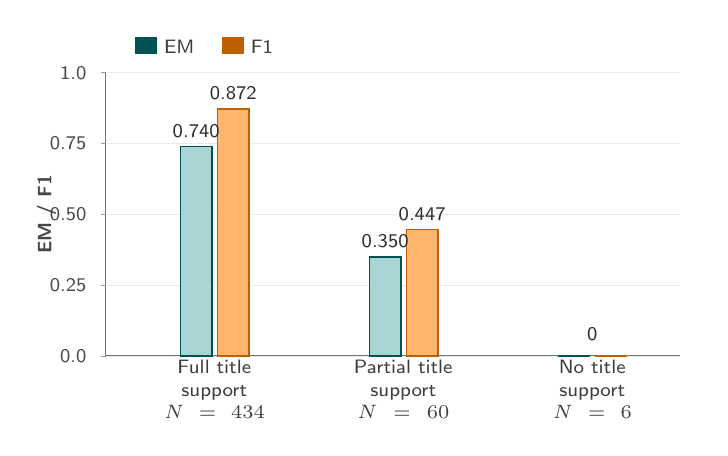
\begin{tikzpicture}[
    font=\sffamily\footnotesize,
    axis/.style={draw=black!55, line width=0.55pt},
    tick/.style={draw=black!40, line width=0.45pt},
    grid/.style={draw=black!8, line width=0.35pt},
    axislabel/.style={font=\sffamily\bfseries\scriptsize, text=black!72},
    barlabel/.style={font=\sffamily\scriptsize, align=center, text=black!76},
    value/.style={font=\sffamily\scriptsize, text=black!82},
    legend/.style={font=\sffamily\scriptsize, align=left, text=black!76}
]

% Supporting-title buckets and answer quality.
\begin{scope}[shift={(0,0)}]
    \draw[axis] (0,0) -- (7.3,0);
    \draw[axis] (0,0) -- (0,3.6);
    \foreach \y/\lab in {0/0.0,0.9/0.25,1.8/0.50,2.7/0.75,3.6/1.0} {
        \draw[tick] (-0.06,\y) -- (0,\y);
        \node[anchor=east, font=\sffamily\scriptsize, text=black!70] at (-0.12,\y) {\lab};
        \draw[grid] (0,\y) -- (7.3,\y);
    }
    \node[rotate=90, axislabel] at (-0.75,1.8) {EM / F1};

    % HyDE full title support: EM=.7396, F1=.8720
    \fill[teal!34] (0.95,0) rectangle (1.35,2.663);
    \draw[teal!65!black, line width=0.55pt] (0.95,0) rectangle (1.35,2.663);
    \fill[orange!58] (1.42,0) rectangle (1.82,3.139);
    \draw[orange!75!black, line width=0.55pt] (1.42,0) rectangle (1.82,3.139);
    \node[value] at (1.15,2.86) {0.740};
    \node[value] at (1.62,3.34) {0.872};
    \node[barlabel, text width=27mm] at (1.38,-0.42) {Full title\\support\\$N=434$};

    % HyDE partial title support: EM=.3500, F1=.4472
    \fill[teal!34] (3.35,0) rectangle (3.75,1.260);
    \draw[teal!65!black, line width=0.55pt] (3.35,0) rectangle (3.75,1.260);
    \fill[orange!58] (3.82,0) rectangle (4.22,1.610);
    \draw[orange!75!black, line width=0.55pt] (3.82,0) rectangle (4.22,1.610);
    \node[value] at (3.55,1.46) {0.350};
    \node[value] at (4.02,1.81) {0.447};
    \node[barlabel, text width=28mm] at (3.78,-0.42) {Partial title\\support\\$N=60$};

    % HyDE no title support: both metrics are zero; the small bucket is labeled without extra decimals.
    \draw[teal!65!black, line width=0.55pt] (5.75,0) -- (6.15,0);
    \draw[orange!75!black, line width=0.55pt] (6.22,0) -- (6.62,0);
    \node[value] at (6.18,0.28) {0};
    \node[barlabel, text width=25mm] at (6.18,-0.42) {No title\\support\\$N=6$};

    \node[legend, anchor=west] at (0.25,3.95) {\textcolor{teal!65!black}{\rule{8pt}{6pt}} EM \quad \textcolor{orange!75!black}{\rule{8pt}{6pt}} F1};
\end{scope}

\end{tikzpicture}%
}
\caption{Supporting-title completeness and answer quality on HotpotQA. The figure groups HyDE-style RAG examples by retrieved supporting-title completeness and reports EM/F1 within each bucket. Full title support means that all annotated supporting titles are retrieved in the top-10 evidence set. The no-title-support bucket contains only six examples and is reported descriptively. The single-annotator EM-mismatch taxonomy is reported separately in the supplement as a descriptive diagnostic.}
\label{fig:evidence_error_taxonomy}
\end{figure*}


\subsection{LLM-Call Accounting}
\label{sec:call_accounting_safety}

Structural call accounting is reported in the supplement rather than repeated as a main-text table. Dense, BM25, Hybrid, Multi-query, and the rule-based evidence-expanded iterative control each use one reader call per question, while Single-query Reformulation and HyDE-style RAG add one query-side generation call. Thus HyDE-style RAG uses 2.00 LLM calls per question and 1000 total LLM calls for the 500-example HotpotQA study. Multi-query and rule-based iterative retrieval do not add LLM calls but execute more retrieval queries per question; provider-side latency and billing are left to future cost instrumentation. The guarded canonicalization selector, guard decomposition, and single-annotator EM-mismatch taxonomy are reported only as supplemental diagnostics.

\subsection{Artifact-Grounded Case Studies}
\label{sec:case_studies}

Three examples selected from rule-filtered candidates using frozen per-example artifacts make the main mechanisms inspectable (Table~\ref{tab:qualitative_cases}). Each case is linked to existing Dense or HyDE reader outputs, supporting-title retrieval states, and HyDE overlap diagnostics.

\begin{table*}[t]
\centering
\caption{Artifact-grounded qualitative case studies emphasizing HyDE retrieval.}
\label{tab:qualitative_cases}
\scriptsize
\begin{threeparttable}
\setlength{\tabcolsep}{3pt}
\begin{tabularx}{\textwidth}{>{\raggedright\arraybackslash}p{0.17\textwidth}
                            >{\raggedright\arraybackslash}p{0.27\textwidth}
                            >{\raggedright\arraybackslash}p{0.23\textwidth}
                            >{\raggedright\arraybackslash}X}
\toprule
Case type & Question summary & Prediction / evidence state & Interpretation \\
\midrule
HyDE evidence acquisition & "Ew!" is a song by a television host born where? & Dense: United States; HyDE: Bay Ridge, Brooklyn; Gold: Bay Ridge, Brooklyn; Dense support partial (1/2); HyDE support full (2/2) & HyDE retrieves the missing supporting title without an exact normalized answer-string match in the hypothetical passage, turning a partial-evidence Dense failure into a correct answer. \\
HyDE evidence acquisition & How many films were directed by the director of Wise Blood? & Dense: I don't know; HyDE: 37; Gold: 37; Dense support partial (1/2), missing John Huston; HyDE support full (2/2) & HyDE retrieves the director page needed for the second hop and turns a partial-support Dense abstention into a correct count answer. \\
Answer-standardization boundary & Which star of Zork was also the voice of Pac-Man? & HyDE: Marty Ingels; Gold: Martin Ingerman; HyDE support full (2/2) & The reader returns the professional name Marty Ingels, whereas the benchmark gold answer uses the birth name Martin Ingerman. The two names refer to the same person, illustrating that exact-match evaluation can count semantically valid aliases as errors. \\
\bottomrule
\end{tabularx}
\begin{tablenotes}
\footnotesize
\item Cases were selected from rule-filtered candidates using frozen HotpotQA per-example artifacts: Dense and HyDE reader outputs, supporting-title states, and HyDE answer-overlap audit rows. They are illustrative rather than additional evaluation examples.
\end{tablenotes}
\end{threeparttable}
\end{table*}


The first two cases show the intended HyDE-style retrieval effect. For a question asking where the host associated with the song ``Ew!'' was born, Dense RAG retrieves only one of the two required supporting titles and answers with an over-broad country; HyDE-style retrieval recovers both supporting titles and the reader returns the exact gold location, even though the generated hypothetical passage does not contain the normalized gold answer string. For the Wise Blood counting question, Dense retrieval misses the director page and the reader abstains, while HyDE retrieves both the film and director pages and the reader returns the correct count.

The final case is an answer-standardization boundary rather than a retrieval failure. In the Zork/Pac-Man example, HyDE retrieves all supporting titles and returns the professional name ``Marty Ingels,'' while EM expects the birth name ``Martin Ingerman.'' The case illustrates why answer-format and alias diagnostics remain useful, but the main mechanism shown by the case studies is still improved evidence acquisition.

\subsection{Secondary Generalization Check}
\label{sec:2wiki_generalization}

The 2WikiMultihopQA experiment tests whether the same supporting-title completeness pattern appears on a second released processed split without retuning the reader prompt (Table~\ref{tab:2wiki_generalization}). For the primary 2Wiki evaluation, no query-generation prompt, retrieval parameter, reader instruction, or query-composition choice was selected using 2WikiMultihopQA results, so this experiment serves as an external check on the retrieval conclusion rather than as a tuning split. This split is harder for complete supporting-title retrieval: one-step Dense RAG retrieves at least one supporting title for 98.4\% of examples but all supporting titles for only 35.8\%. HyDE-style RAG raises all-support hit@10 to 0.6680 and mean recall@10 to 0.8575, and it improves reader performance to EM/F1 = 0.6620/0.7289, compared with 0.5400/0.5767 for Dense and 0.5840/0.6220 for Hybrid.

The paired 2Wiki checks in Supplement Table~\ref{supp:tab:2wiki_paired_statistics} show the same direction. Against Dense RAG, HyDE improves all-support hit@10 by +0.3100 [0.2680, 0.3520] and F1 by +0.1523 [0.1186, 0.1881]. Against Hybrid RAG, it improves all-support hit@10 by +0.2200 [0.1800, 0.2620] and F1 by +0.1069 [0.0751, 0.1399]. The 2Wiki answer-string diagnostic is reported in Supplement Section~\ref{supp:sec:supp_answer_overlap_normalization}.

\section{Discussion and Limitations}
\label{sec:discussion_limitations}

HyDE-style document-like query expansion is associated with improved multi-hop supporting-evidence acquisition under the processed local-corpus protocol studied here. This framing is intentionally empirical: the paper does not claim HyDE itself as a new algorithm, but uses a controlled protocol to test when document-like expansion helps complete supporting-title and paragraph-text retrieval. On both HotpotQA and 2WikiMultihopQA, the observed gain appears first in complete supporting-title retrieval and then in reader EM/F1. Paired retrieval tests, paired answer tests, and supporting-title completeness buckets point in the same direction: examples with all supporting titles retrieved are much easier for the reader than partial-title-support or no-title-support examples. A supporting-paragraph audit over \texttt{is\_supporting=true} corpus records gives identical all-support and recall values for the audited rows listed in Supplement Table~\ref{supp:tab:supporting_paragraph_audit}, reducing the concern that the title metric is inflated by retrieving the right page name but the wrong processed paragraph. Because each annotated supporting title maps to one supporting paragraph record in these released processed splits, the audit is best read as an exact record-recovery check rather than as independent sentence-level evidence. The central empirical message is therefore that supporting-title completeness, aligned with paragraph-text recovery in the processed artifacts, is a major observed bottleneck under the evaluated protocol.

The mechanism evidence is bounded. The matched-call rewrite and equal-budget diagnostics rule out ``one extra LLM call'' and generated length as sufficient explanations, but they do not show that document-like organization universally dominates every high-information query form. Document-like passages improve over direct rewrite and decomposition in the equal-budget diagnostic, while the comparison with keyword/entity expansion is dataset-dependent. The targeted Qwen-Turbo readout gives the same caution downstream: it is positive over direct rewrite but mixed against keyword/entity expansion. We therefore interpret the result as a retrieval-stage advantage of document-like organization over ordinary rewriting and decomposition under this generator, encoder, and local-corpus protocol, not as a reader-independent or universal end-to-end superiority claim.

The guarded canonicalization diagnostic is deliberately secondary: it changes HyDE-style RAG by only +0.0040 EM and +0.0030 F1, is not significant under McNemar's paired EM test ($p=0.5000$), and is reported in the supplement as an answer-format risk analysis rather than as a main contribution.

The main boundary conditions are concentrated in the threats-to-validity analysis below: answer-string overlap in generated query text, the processed local-corpus protocol rather than full-wiki retrieval, and structural rather than latency-measured cost accounting.

\subsection{Threats to Validity}
\label{sec:threats_to_validity}

\textbf{Construct validity.} The evaluation uses supporting-title hit@10, mean supporting-title recall@10, EM, and token F1 as operational measures of evidence acquisition and answer quality. These metrics fit the processed multi-hop QA protocol, but they do not capture all forms of evidence usefulness or answer correctness. The added supporting-paragraph audit tightens the retrieval unit from title to exact normalized title--paragraph text and finds no title-versus-paragraph discrepancy in the audited rows listed in Supplement Table~\ref{supp:tab:supporting_paragraph_audit}; because the released processed splits provide one supporting paragraph record per annotated supporting title, this audit primarily verifies exact processed-record recovery. However, the processed 500-example JSONL artifacts used here do not expose gold supporting sentence text, so we cannot measure supporting-fact sentence coverage or within-paragraph grounding quality. EM and token F1 can also penalize acceptable aliases. The EM-mismatch analysis and qualitative cases make these boundaries visible, but the taxonomy is a single-annotator diagnostic without independent agreement measurement and is not a substitute for systematic human factuality annotation.

\textbf{Internal validity.} The main internal risk is query-side answer-string overlap from the hypothetical passage. This risk is related to recent evidence that LLM-based hypothetical-document expansion can reproduce benchmark knowledge in the generated query text \cite{yoon2025knowledgeleakage}. Many generated hypothetical passages contain the normalized gold answer string: 292/500 on HotpotQA and 347/500 on 2WikiMultihopQA. The reader-only evidence boundary prevents the generated passage from being used as reader evidence, but the passage can still contain answer-like strings and influence which corpus documents are retrieved. Exact answer-absent, gold-content-stratified, and gold-aware scrubbed retrieval diagnostics reduce the explanation that HyDE gains come only from exact normalized answer-string overlap. They also show that answer-like strings and supporting-entity mentions contribute to the full gain. These diagnostics cannot rule out paraphrased answer content, parametric memory, benchmark contamination, or other semantic gold-evidence traces in the query generator.

The token-matched audit truncates existing HyDE passages rather than independently generating equal-length hypothetical passages. It therefore measures sensitivity to information removal rather than providing a clean causal comparison of textual form at equal generation length. The new independent equal-budget diagnostic reduces this limitation for retrieval metrics, but it cannot fully equalize entity count, factual density, or parametric knowledge in generated text, and it does not test reader sensitivity to the retrieved evidence.

A second internal-validity risk is configuration selection and experiment timing. The reported prompt and result artifacts are frozen for audit and rescoring, but not every design choice was selected on a separate development split or before the first HotpotQA result analysis. We therefore distinguish three evidence tiers. The primary frozen study is the original MiniLM-based HotpotQA retrieval-reader comparison with the main lightweight baselines, HyDE query generation, matched-call direct rewriting control, top-$k=10$ evidence budget, and Qwen3.7-Max reader. The BGE-base reproduction, equal-budget 40-word query-form diagnostic, gold-aware scrubbing, corpus-scale and hard-negative audits, top-$k$ sensitivity, supporting-paragraph audit, and Qwen-Turbo fixed-evidence reader check are post-hoc robustness diagnostics added after the primary results to test specific threats to validity. The equal-budget prompts were designed after observing the primary HotpotQA pattern; after the prompt family was fixed, it was applied unchanged to both HotpotQA and 2WikiMultihopQA, making 2Wiki a no-retuning secondary check for that diagnostic rather than a fully independent pre-registered validation. Finally, verifier risk rules and deterministic guards were informed by diagnostics on the reported processed HotpotQA split before final artifact freezing. The verifier-backed canonicalization analysis should therefore be read as an exploratory safety and answer-standardization study, not as evidence of independently tuned verifier generalization.

\textbf{External validity.} The experiments use released 500-example processed HotpotQA and 2WikiMultihopQA splits with local candidate evidence pools. This makes paired comparison and artifact freezing practical, but it is not a full-wiki retrieval setting. The stronger-encoder robustness check, the 50k/100k processed-train distractor stress test, the leakage-filtered and BGE-hard corpus-scale audit, and the top-5/10/20 sensitivity audit reduce the risk that the effect is limited to one weak encoder, the smallest local index, added gold-title leakage, random easy distractors, or a single rank-10 cutoff, but they still do not replace open-domain Wikipedia retrieval. The BGE-hard row is selected from the already audited processed-train 100k pool rather than from all Wikipedia paragraphs, so it tests a harder local negative subset but not the full open-domain retrieval distribution. The implemented comparison rows also have a limited role: BM25, Hybrid, and Dense are lightweight retrieval baselines, while matched-call rewriting, rule-based multi-query retrieval, and rule-based iterative retrieval are mechanism or heuristic controls. They should not be read as faithful public implementations of Query2doc, Rewrite-Retrieve-Read, ReDE-RF, IRCoT, or agentic RAG systems. Results may differ with official or more closely tuned published baselines, other retrievers, different readers, open-weight systems, top-$k$ budgets beyond 20, or datasets with different compositional structure. One targeted Qwen-Turbo readout of fixed equal-budget evidence preserves the document-like answer advantage over direct rewrite on both datasets, while the comparison with keyword/entity expansion is positive on HotpotQA and essentially tied on 2Wiki. This single hosted-reader check is not a broad reader sweep and does not change the paper's retrieval-stage mechanism claim.

\textbf{Reproducibility and cost validity.} Prompts, retrieval files, answer files, analysis scripts, and model invocation ledgers are frozen as project artifacts, but hosted LLM APIs can change over time. The Qwen3.7-Max records document interface, dates, decoding settings, and artifact paths. They do not include provider-side request IDs, exact token accounting for every call, wall-clock latency, or billing exports. The efficiency claim is therefore limited to structural LLM-call counts, retrieval-query executions, and prompt-character counts.

\section{Conclusion}
\label{sec:conclusion}

This paper presented a controlled diagnostic study of HyDE-style document-like generative query expansion in a fixed-depth, training-free protocol for multi-hop RAG. Across HotpotQA and the secondary 2WikiMultihopQA check, the main observed pattern is better complete supporting-title retrieval, with matching paragraph-text audit results and reader EM/F1 gains reported for the fixed reader used in the end-to-end pipeline. The matched-call query-reformulation controls show that the retrieval gain is not explained by an extra query-side LLM call alone. The strict equal-budget retrieval-only diagnostic further shows that independently generated document-like passages outperform direct rewrites on complete supporting-title retrieval at closely matched generated lengths and call budgets. The secondary guarded canonicalization diagnostic remains an answer-format risk analysis rather than part of the main empirical claim.

Overall, the evidence supports a retrieval-stage conclusion: under the evaluated processed local-corpus protocol, document-like hypothetical expansion improves supporting-title and paragraph-text acquisition over direct reformulation and question decomposition at a similar generation budget, while its comparison with keyword/entity expansion is dataset-dependent. The targeted Qwen-Turbo readout is consistent with this boundary rather than a broad reader-independent superiority claim. Sentence-level supporting-fact coverage remains outside the available processed artifacts, and code/artifact availability is described in Supplement Section~\ref{supp:sec:supp_code_artifact_availability}.


\bibliographystyle{plain}
\bibliography{related_work_references}

\end{document}
